\documentclass[12pt,a4paper]{article}

\usepackage[utf8]{inputenc}
\usepackage[english]{babel}

\usepackage[pdftex]{graphicx}
\usepackage[top=1in, bottom=1in, left=1in, right=1in]{geometry}

\linespread{1.06}
\setlength{\parskip}{8pt plus2pt minus2pt}

\widowpenalty 10000
\clubpenalty 10000

\newcommand{\eat}[1]{}
\newcommand{\HRule}{\rule{\linewidth}{0.5mm}}

\usepackage[official]{eurosym}
\usepackage{enumitem}
\setlist{nolistsep,noitemsep}
\usepackage{float}
\usepackage[hidelinks]{hyperref}
% \usepackage{cite}
\usepackage{lipsum}

\usepackage[newfloat]{minted}
\usepackage[skins,minted]{tcolorbox}

\definecolor{mintedbackground}{rgb}{0.97,0.97,0.97}

\newmintedfile[htmlcode]{html}{linenos, breaklines, encoding=utf8, frame=single, framesep=5pt, framerule=0.4pt, bgcolor=mintedbackground,autogobble,numbersep=5pt}

\newmintedfile[csscode]{css}{linenos, breaklines, encoding=utf8, frame=single, framesep=5pt, framerule=0.4pt, bgcolor=mintedbackground,autogobble,numbersep=5pt}

\newmintedfile[xmlcode]{xml}{linenos, breaklines, encoding=utf8, frame=single, framesep=5pt, framerule=0.4pt, bgcolor=mintedbackground,autogobble,numbersep=5pt}

\newmintedfile[phpcode]{php}{linenos, breaklines, encoding=utf8, frame=single, framesep=5pt, framerule=0.4pt, bgcolor=mintedbackground,autogobble,numbersep=5pt}

\newtcblisting{myminted}[3][]{minted language=#3,
    enhanced, listing engine=minted,
    listing only, #1, title=#2, 
    colback=mintedbackground, colbacktitle=mintedbackground, coltitle=darkgray, 
    arc=0pt,outer arc=0pt, 
    boxrule=0mm, 
    toptitle=1mm, bottomtitle=1mm,
    titlerule=1pt, colframe=gray, titlerule style={mintedbackground, dashed}    
}


\newtcbinputlisting[list inside=mypyg]{\codeFromFile}[6][]{%
    listing engine=minted,
    enhanced,
    colback=mintedbackground,
    colbacktitle=mintedbackground,
    coltitle=darkgray,
    arc=0pt,outer arc=0pt,
    boxrule=0mm,
    toptitle=1mm, 
    bottomtitle=1mm,
    titlerule=1pt, 
    colframe=gray,
    minted options={#1},
    minted language=#2,
    listing file={#3},
    title={#4},
    label=#5,
    listing only,
    titlerule style={mintedbackground, dashed},
    #6
}{}

\begin{document}

\begin{titlepage}
    \begin{center}

        % Top 
        
\includegraphics[width=0.25\textwidth]{res/NSUT.png}~\\[0.5cm]
        \textsc{\Large Netaji Subhas University of Technology}\\[2cm]

        % Title
        \HRule \\[0.4cm]
        {
        \LARGE
        \textbf{Practical Report}\\[0.4cm]
        \emph{Microprocessors and Microcontrollers}\\[0.4cm]
        }
        \HRule \\[1.5cm]



        % Author
        { \large
        Kushagra Lakhwani \\[0.1cm]
        \texttt{2021UCI8036}\\[0.5cm]
        Computer Science Engineering (Internet of Things)\\[0.1cm]
        \textit{Semester 3} \\[0.1cm]
        }

        \vfill

        \textsc{\large Department of Computer Science \& Engineering}\\[0.4cm]


        % Bottom
        {\large \today}

    \end{center}
\end{titlepage}

\tableofcontents
\addtocontents{toc}{\protect\thispagestyle{empty}}
\newpage
\setcounter{page}{1}

% \section{Introduction}\label{sec:intro}
\lipsum[2]\cite{einstein}
\pagebreak


\section{Using HTML}\label{sec:intro}


\section{CSS}\label{sec:css}

\subsection{Project}

\subsubsection*{Project Description}

This is a simple web-page that utilizes an external cascade stylesheet

\subsubsection*{Project Showcase}
\begin{figure}[H]
    \centering
    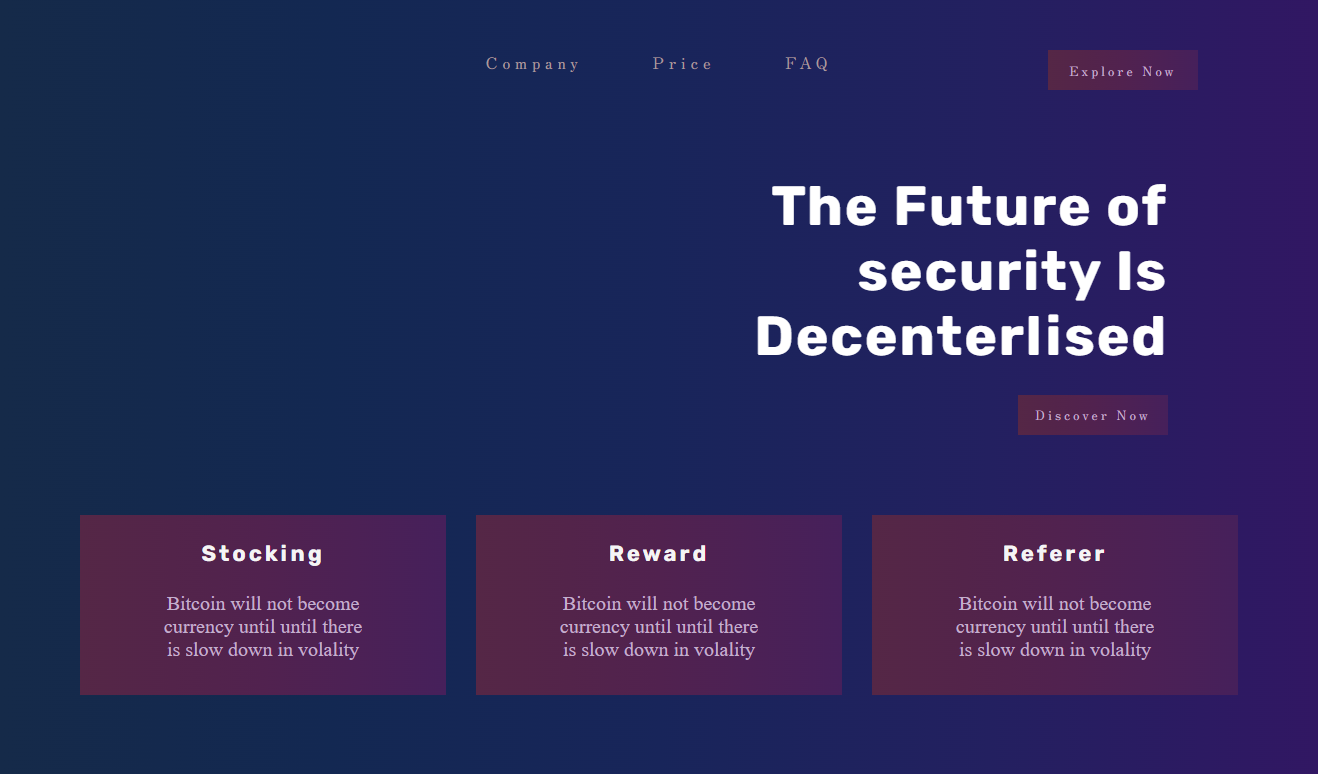
\includegraphics[width=0.8\textwidth]{res/styled-page.png}
    \caption{Styled Web page}
    \label{fig:css-page}
\end{figure}

\subsection{Source Code}

\inputminted[
    linenos,
    breaklines,
    encoding=utf8,
    label=page.html,
    framesep=2mm,
    frame=leftline,
    numbersep=5pt,
]{css}{"./code/page.css"}

% \begin{myminted}{/files/location/on/system.sh}{bash}
%     #!/bin/bash
%     echo "I am a bash file"
% \end{myminted}

\codeFromFile{css}{./code/page.css}{page.css}{page.css}{}

\texttt{page.html}
\inputminted[linenos, breaklines, encoding=utf8,label=page.html]{html}{"./code/page.html"}

\pagebreak

\section{Form With Validation}\label{sec:form}

\subsection{Project}

\subsubsection*{Project Description}

This project is a \textit{Signup form with validation.}

\subsubsection*{Project Showcase}
\begin{figure}[H]
    \centering
    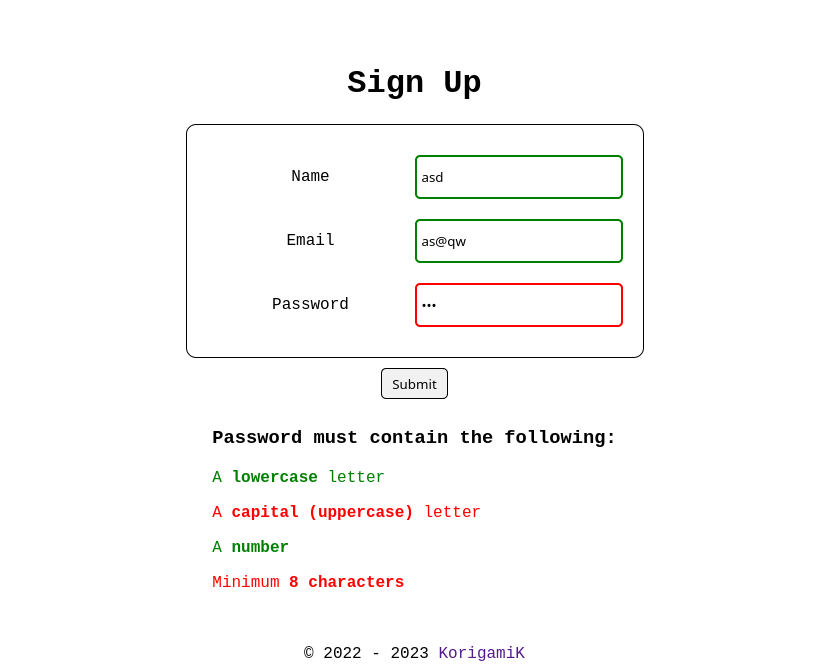
\includegraphics[width=0.8\textwidth]{res/form.png}
    \caption{Form With Validation}
    \label{fig:form}
\end{figure}

\subsection{Source Code}

File: \texttt{form.html}
\htmlcode{./code/form.html}

\section{Using HTML, CSS \& JavaScript}\label{sec:todo}

\subsection{Project}

\subsubsection*{Project Description}

This is a minimal To-do List application written in HTML, CSS and JavaScript. It is a single page application that allows the user to add, edit and delete tasks.

The tasks are added though a form that is displayed at the top of the page.
The tasks are displayed in an unordered list below the form. And a delete button is displayed next to each task.
The click and submit events are handled by JavaScript functions.

\subsubsection*{Project Showcase}

\begin{figure}[H]
    \centering
    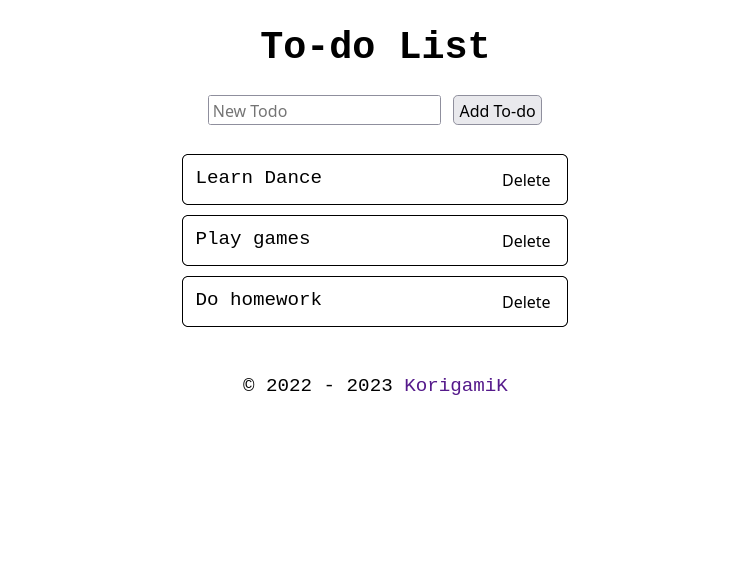
\includegraphics[width=0.8\textwidth]{res/todo-list.png}
    \caption{To-do List App}
    \label{fig:todo-list}
\end{figure}


\subsection{Source Code}

File: \texttt{todo-list.html}
\htmlcode{./code/todo-list.html}

\section{XML}\label{sec:xml}

\subsection{Project}

\subsubsection*{Project Description}

This is a syndication feed for my blog written in \textit{XML} following the \href{http://www.w3.org/2005/Atom}{Atom} standard for syndication.


\subsection{Source Code}

File: \texttt{feed.xml}
\xmlcode{./code/feed.xml}

\section{PHP}\label{sec:php}

\subsection{Project}

\subsubsection*{Project Description}

This is a simple \textit{PHP} application\cite[GitHub]{php-fruits} that displays a list of fruits. The fruits are stored in a SQLite database.

The user can add more fruits to the list by filling a form and submitting it and the user can also buy the fruits by clicking on the \textit{Buy} button.

The fruit is removed from the list when none of its kind are left.

\subsubsection*{Project Showcase}

\begin{figure}[htbp]
    \centering
    \includegraphics[width=0.8\textwidth]{./code/php-fruits/screenshots/home.png}
    \caption{PHP Fruits App}
    \label{fig:php}
\end{figure}


\subsection{Source Code}

File: \texttt{index.php}
\phpcode{./code/php-fruits/index.php}

File: \texttt{app.php}
\phpcode{./code/php-fruits/app.php}

\pagebreak

File: \texttt{api/add.php}
\phpcode{./code/php-fruits/api/add.php}

File: \texttt{api/buy.php}
\phpcode{./code/php-fruits/api/buy.php}


\pagebreak

\bibliographystyle{ieeetr}
\bibliography{refs}
\listoffigures

\end{document}
